%
%   Copyright 2013 Katarzyna Szawan <kat.szwn@gmail.com>
%       and Michał Rus <m@michalrus.com>
%
%   Licensed under the Apache License, Version 2.0 (the "License");
%   you may not use this file except in compliance with the License.
%   You may obtain a copy of the License at
%
%       http://www.apache.org/licenses/LICENSE-2.0
%
%   Unless required by applicable law or agreed to in writing, software
%   distributed under the License is distributed on an "AS IS" BASIS,
%   WITHOUT WARRANTIES OR CONDITIONS OF ANY KIND, either express or implied.
%   See the License for the specific language governing permissions and
%   limitations under the License.
%

\section{Android application}
\label{sec:android-app}

\subsection{Navigation}
\label{subsec:drawing}
The first step in creating an Android application was writing of the basic views. According to the project, our application should consist of two `views': the first with list of mind maps and the second, with a view of a single map. Both views share an Action Bar with action buttons (which, for example, open a file, close a map, add a new map) and application's name and icon, as well as a navigation bar with tabs.

\subsubsection{Action Bar}
\label{subsubsec:action-bar}
For most Android applications, a basic component is an Action Bar. It is one of the most important design elements due to the fact, that most Android applications share it. Due to this consistency, a potential user is instantly familiar with application's basic interface.

There are a number of things that can be put inside Action Bar, for example: a search bar, action buttons etc. In our application, we added the components listed below.

\begin{itemize}
	\item Button for importing an existing mind map  from an XMind file (in a main view with list of available maps).
	\item Button for adding a new mind map (in a main view with list of available maps).
	\item Button for closing an opened mind map (in a single map view).
	\item Navigation bar which consists of tabs with opened maps (default tab is a view with list of available maps).
\end{itemize}

We wanted our application to be runnable even on older Android version, so instead of regular system-provided ActionBar library, we decided to use support libraries, which take care of backward compatibility from 2.x Android versions up.

ActionBarSherlock is an standalone library designed to simplify the use of the Action Bar in all versions of Android through a single API. The library will automatically use the native \inlinecode{ActionBar} implementation on Android 4.0 or later \cite{Wharton:2013:sherlock}. Using it is fairly simple: the main difference lies in names of \inlinecode{ActionBar} classes and methods. Most of them are prefixed with `Sherlock-' (for example: \inlinecode{SherlockActivity, SherlockFragmentActivity, SherlockFragmen} etc.). The same goes for imports.

\subsubsection{Bidirectional ScrollView}
\label{subsubsec:action-bar}
Our application's most important feature---creating mind maps---requires a convenient way of navigating through a map. It should support multi-directional scrolling. In Android API there is no class which can handle multi directional scrolling (to discourage this for performance reasons). Some classes, like \inlinecode{TextView} or \inlinecode{ListView}, have vertical scrolling implemented, but generally, scrolling is handled by two classes extending \inlinecode{android.widget.FrameLayout}: \inlinecode{HorizontalScrollView} and \inlinecode{ScrollView}. Implementing bidirectional scroll view was one of the problems we encountered while writing the Android application. Our solution is described in \cref{subsec:problem-scrollview}.

\begin{figure}[h]
	\centering
	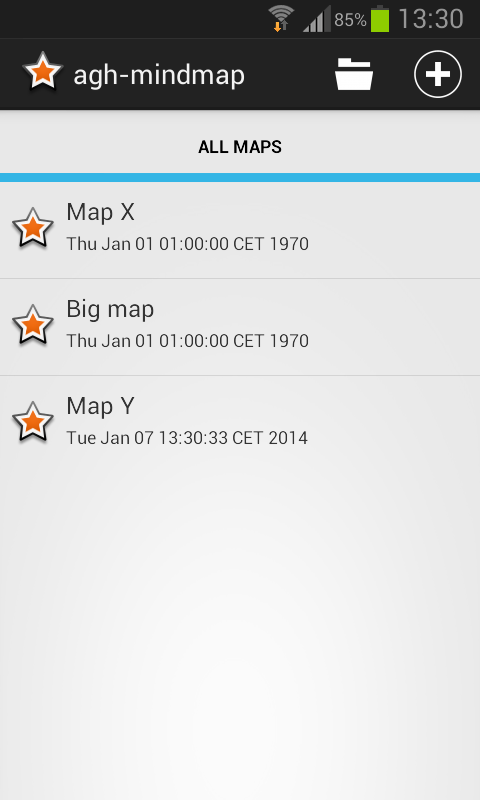
\includegraphics[width=.5\textwidth]{graphics-screenshot-list}
	\caption{View of a mind map list, initial screen.}
	\label{fig:screen-maplist}
\end{figure}

\subsection{Drawing mind maps}
\label{subsec:drawing}
In the next stage of work, we focused on a single mind map view. The main components used in drawing here are: \inlinecode{NodeView}, representing a single mind node, and \inlinecode{ArrowView} which serves as a line connecting the mind nodes. They are placed in the \inlinecode{MindFragment}. Every \inlinecode{NodeView} is paired with a \inlinecode{SubtreeWrapper}, which acts as a `container' holding the mind node and all its children.

\inlinecode{NodeView} is implemented as extending \inlinecode{FrameLayout}. It extends a \inlinecode{ViewGroup}, and we chose it because mind node's view have two children: a text field with node's content and a button. \inlinecode{FrameLayout} can be used as a parent for multiple children and it can control their position within the \inlinecode{ViewGroup} by assigning gravity to each child with the \inlinecode{android:layout\_gravity} attribute. Child views are drawn in a stack, with the latest added child on top \cite{API:2013:fl}.

Arrow is implemented as a single View with custom onDraw method. It connects a mind node with its parent. If a mind node has multiple children, then lines coming out of the child nodes are connected in one point and then a single line goes to the parent node. It makes the whole map more readable.

In order to keep the code readability, we refactored the process of drawing out to a separate class, \inlinecode{MapPainter}, whose constructor is called in the \inlinecode{onCreateView} method of the \inlinecode{MapFragment}. This class provides all necessary values and methods needed to draw a mind map:

\begin{itemize}
	\item canvas padding and subtree margin,
	\item the horizontal distance between child nodes,
	\item \inlinecode{arcShortRadius} which determines the radius depending on the number of children which is used later in map painter to calculate the position of mind node on the X axis,
	\item \inlinecode{nodeViewSize} setting the size of a mind node,
	\item \inlinecode{initializeNodeView} which initializes inflated mind node layout,
	\item \inlinecode{updateNodeView} setting the content of a mind node.
\end{itemize}

As soon as other elements are prepared, \inlinecode{HorizontalScrollView} and its inner \inlinecode{ScrollView} layouts are found and set, current mind map is found by UUID and the paper layout is set, a map painter is called.

When it comes to the positioning, it was one of the most difficult tasks we faced. \inlinecode{MapPainter} handles calculating the position of mind nodes and arrows. It also manages \inlinecode{SubtreeWrappers} and their accordance with \inlinecode{NodeViews}. It can update the size and coordinates of mind nodes, as well as remove them, or recalculate nodes' positions. As far as the order of the children is concerned, there is a field in MindNode model, \inlinecode{initialOrdering}, and it is set when children are created. A detailed description can be found in \cref{subsec:problem-positioning}.

\subsection{Creating, editing and removing mind nodes}
\label{subsec:drawing}
Managing the mind nodes is fairly simple. There are three actions a user can perform: create a `child' mind node, delete a node (with its whole subtree) and edit node's content. 

\subsubsection{Creating a child mind node}
\label{subsubsec:create-child}
In order to create a child mind node, one must click on a plus button located on the outer part of the parent node. It is implemented in the \inlinecode{addChildNode} method of \inlinecode{MapFragment} class. It calls \inlinecode{createChildOf} method from \inlinecode{MindNode} object and then repaints the map using an instance of \inlinecode{MapPainter}.

\subsubsection{Deleting a mind node with its subtree}
\label{subsubsec:delete-node}

Deleting a node with its subtree can be performed by long-clicking on this node. It is implemented in the \inlinecode{removeNode} method of the \inlinecode{MapFragment}. It also calls a \inlinecode{remove} method from \inlinecode{MindNode} class, which uses \inlinecode{deleteChildrenOf} a private method from the \inlinecode{MindNode} object. It also clears node's content and schedules asynchronous update with the \inlinecode{Synchronizer} class.
 
\subsubsection{Editing a mind node's content}
\label{subsubsec:delete-node}
A user can edit node's content by clicking on node's body. It is possible thanks to setting two listeners while initializing a \inlinecode{NodeView}: an \inlinecode{OnEditorActionListener} and an \inlinecode{OnFocusChangeListener}. The actual change of the content is performed while handling an onFocusChange event.

\begin{figure}[h]
	\centering
	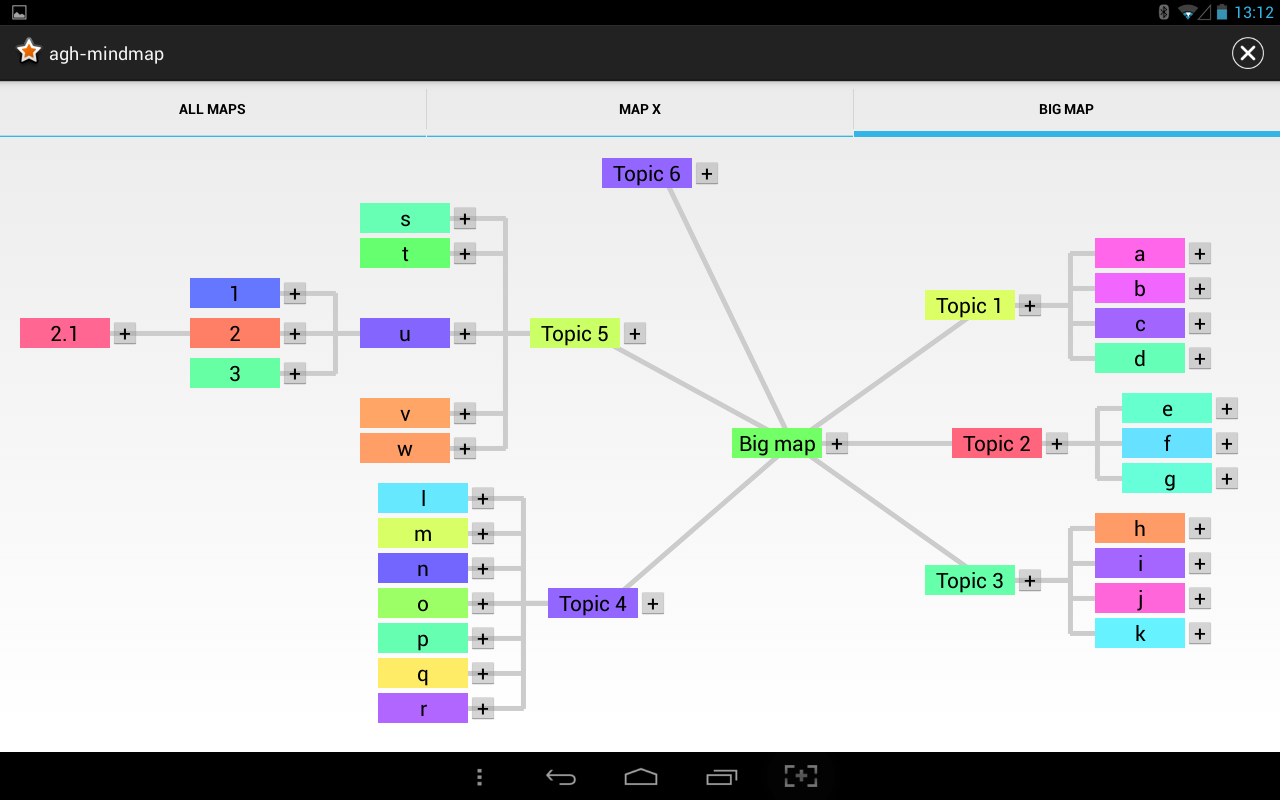
\includegraphics[width=\textwidth]{graphics-screenshot-big-map}
	\caption{View of a mind map.}
	\label{fig:screen-map}
\end{figure}

\subsection{Importing from existing .xmind files}
\label{subsec:import}
Processing the given .xmind file has gone according to the project. We implemented the basic version of importing which does not take into consideration the extra information which is provided in a standard .xmind file. We load only the structure of a mind map, the content of all nodes and their order. A single XMind file can have multiple sheets, meaning multiple mind maps. Handling this feature is, too, implemented (as a result of importing a multi-sheet file, we get multiple maps, one for each sheet).

As we supposed, Scala turned out to be very handy in processing XML files. A method for extracting a single mind map from an XMind sheet has only 5 lines:
\begin{verbatim}
def extractor(topic: Node, parent: MindNode) {
  (topic \textbackslash "children" \ "topics" \ "topic").zipWithIndex.foreach {
    case (childXml, i) =>
      val child = MindNode.createChildOf(parent, i.toDouble)
      child.content = Some((childXml \ "title").head.text)
      extractor(childXml, child)
  }
}\end{verbatim}

Here is a short explanation of the above excerpt. A single topic represents a node and root's children nodes are imported recursively. As we described in \cref{subsec:xmind-exchange}, one can navigate through the data using \inlinecode{\textbackslash} and \inlinecode{\textbackslash\textbackslash} operators, meaning, respectively, `search in direct children' and `search in all subtags.' While creating a node, we are setting ordering, here derived from index \inlinecode{i}. A content of a tag can be accessed its \inlinecode{text} method.

\begin{figure}[h]
	\centering
	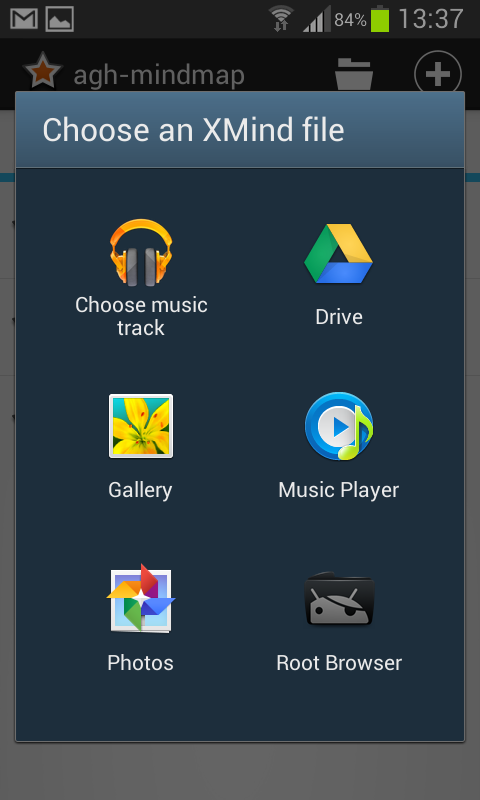
\includegraphics[width=.5\textwidth]{graphics-screenshot-import}
	\caption{View of a file chooser, importing an existing .xmind file.}
	\label{fig:screen-filechooser}
\end{figure}

\subsection{User interface}
\label{subsec:ui}
Thanks to multi-directional scrolling it is easy to navigate even if the map is too big to be fit on user's screen.

\todo[inline]{\kasia{Why we designed UI in such a way.}}